%% CAPITULO 3
\hypertarget{estilo:capitulo}{}
\chapter{IMPACTO DA ASSIMILAÇÃO DE PRECIPITAÇÃO NO SISTEMA Eta+RPSAS}
\label{ss:cap3}

\section{Avaliação das médias dos experimentos durante Janeiro de 2003}
\label{ss:avalmedia}

Para se verificar o comportamento dos experimentos (sumarizados na \autoref{tab04}) ao longo do período de integração do modelo (de 02 a 30 de Janeiro de 2003), foi feita uma avaliação espacial e temporal média da integração do modelo durante o período de estudos em comparação com a Reanálise 2 do NCEP/DOE e a Reanálise do CPTEC. Para esta avaliação foram consideradas as análises do sistema RPSAS em um total de 113 análises (entre 00Z, 06Z, 12Z e 18Z, considerando-se também  o período de spin up), a partir das quais foi feita a média espacial para o domínio de integração do modelo. Todos os campos considerados nesta avaliação espacial (incluindo-se a reanálise do CPTEC) foram interpolados para a grade da reanálise do NCEP utilizando-se a função \textit{lterp} do GrADS. 

Na \autoref{ss:avalanl} é apresenta a avaliação espacial das Análises do sistema RPSAS contra as reanálises do CPTEC e do NCEP. Foram avaliadas as variáveis Temperatura, Ventos (componentes $u$ e $v$), Altura Geopotencial e Circulação do Vento (Linha de Corrente) nos níveis de 850, 500 e 250 hPa. Também, foram verificadas separadamente as componente zonal do vento ($u$) em 250 hPa e meridional ($v$) em 850 hPa, além da Temperatura a dois metros. Na \autoref{ss:avalesanl} é feita uma avaliação do Viés e do Erro Quadrático Médio das séries das análises do RPSAS contra a reanálise do NCEP para o período de estudos. Em seguida na \autoref{ss:avaltempumi}, é feita uma análise média da temperatura e da umidade do solo do período. Na \autoref{ss:avalprev} são apresentas as avaliações das previsões do modelo Eta contra as observações do SALLJEX, GPCP e TRMM. Esta avaliação é feita para as mesmas variáveis, além da previsão de precipitação.

\subsection{Avaliação das Análises (Análises RPSAS X Reanálises)}
\label{ss:avalanl}

A \autoref{fig10} mostra os campos interpolados médios de Linha de Corrente para o nível de 850 hPa. Em a) tem-se o experimento SAP, em b) o experimento CAP, em c) a Reanálise do CPTEC e em d) a Reanálise 2 do NCEP/DOE (as demais figuras presentes nesta seção, seguem a mesma ordem de apresentação).

Comparando-se os dois experimentos (SAP e CAP), nota-se que em ambas as simulações o padrão de escoamento é semelhante a partir do qual pode-se observar um gradiente do escoamento de leste sobre o Atlântico Subtropical e outro de oeste sobre o norte da AS. Em relação à reanálises, a do CPTEC também apresenta estes dois gradientes com um padrão de circulação mais organizado apresentando também um giro ciclônico bem definido sobre o Atlântico Subtropical dando suporte a esse escoamento de leste. Na reanálise do NCEP também observa-se esta confluência do escoamento de leste sobre o Atlântico Subtropical, e também o de oeste sobre o Norte da AS, porém um pouco menos intenso. Ambos os experimentos tenderam a simular uma circulação ao centro do continente, sendo esta mais bem caracterizada no experimento CAP. Este tipo de circulação ciclônica simulada pelo experimentos, pode ter sido causada pela tendência dos experimentos em apresentar maiores valores de temperatura à superfície (Temperatura à dois metros), o que pode ser observado na \autoref{fig11}. Neste caso os experimentos SAP e CAP apresentam valores mais elevados da temperatura em relação à reanálises. Além disso, as reanálises também divergem entre si no que se refere aos gradientes de temperatura que podem ser observados nas imagens da \autoref{fig11}. 

Este tipo de circulação apresentada pelos experimentos SAP e CAP é refletido em níveis mais altos, especialmente em 250 hPa (\autoref{fig12}) em que o sentido do giro é contrário ao que ocorre em superfície. Este fenômeno pode ser observado nos quatro casos (nos dois experimentos e nas duas reanálises), porém com a diferença de que a reanálise do NCEP apresenta um vórtice anti-ciclônico bem definido, em comparação com os outros campos de circulação neste mesmo nível. Observa-se também que esta diferença é mais tênue em relação à reanálise do CPTEC, cujo campo de temperatua em altos níveis (250 hPa – \autoref{fig13}) é mais semelhante ao da reanálise do NCEP.

\begin{figure}[!hbp]
\centering
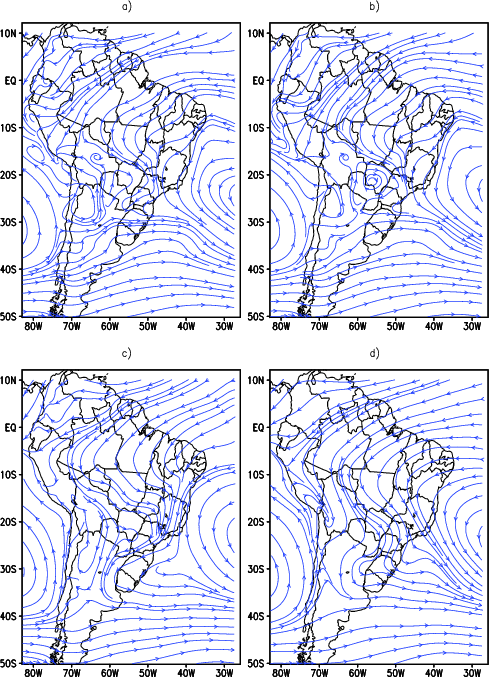
\includegraphics[height=15cm]{./figs/media_corrente_anl_850hPa.png}
\caption{Linha de Corrente para o nível de 850 hPa. a) experimento SAP, b) experimento CAP, c) Reanálise CPTEC, d) Reanálise 2 NCEP/DOE. As unidades estão em ms-1.}
\label{fig10}
\end{figure}

Além disso, o padrão de circulação mostrado na \autoref{fig10}, mostra que existe um corredor de vento que é mais bem caracterizado pelas reanálises do que pelos experimentos. Este corredor de vento, mostrado na \autoref{fig15} (mais adiante) é característico do JBN. 

\begin{figure}[!hbp]
\centering
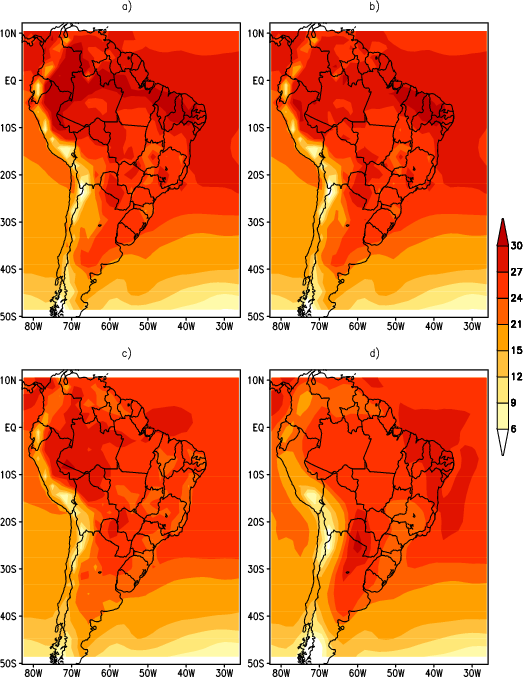
\includegraphics[height=15cm]{./figs/media_tp2m_anl.png}
\caption{Idem à \autoref{fig10}, para a Temperatura doa Ar à Superfície (T2M). As unidades estão em ºC.}
\label{fig11}
\end{figure}

\begin{figure}[!hbp]
\centering
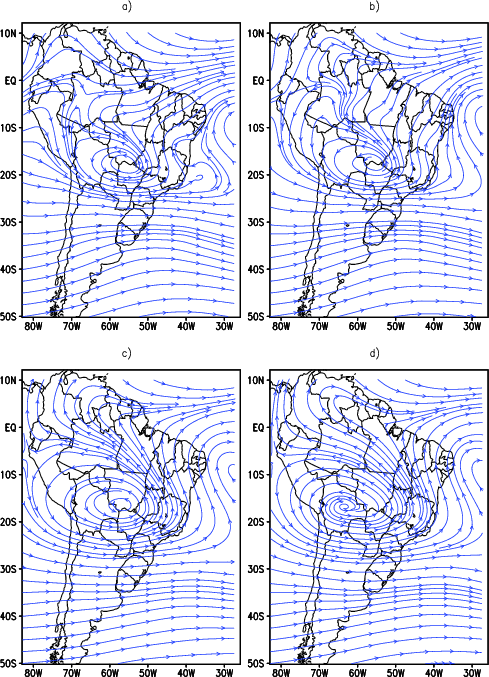
\includegraphics[height=15cm]{./figs/media_corrente_anl_250hPa.png}
\caption{Idem Figura 10, para o nível de 250 hPa. As unidades estão em ms-1.}
\label{fig12}
\end{figure}


\begin{figure}[!hbp]
\centering
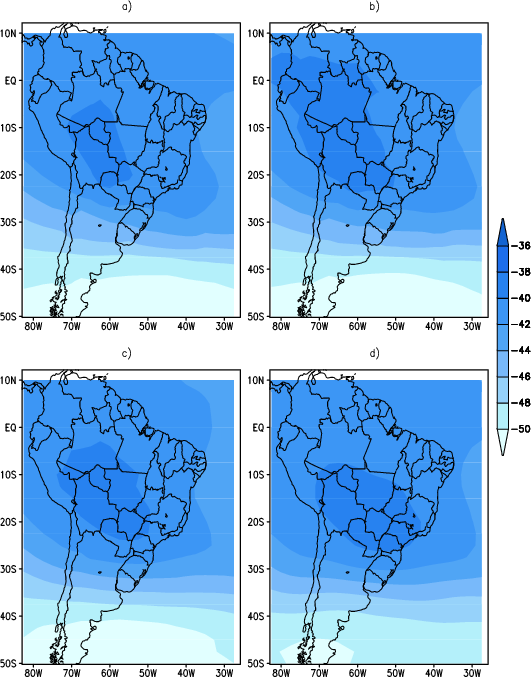
\includegraphics[height=15cm]{./figs/media_temp_anl_250hPa.png}
\caption{Temperatura do Ar para o nível de 250 hPa. As unidades estão em ºC.}
\label{fig13}
\end{figure}

Em níveis médios (500 hPa – \autoref{fig14}), os experimentos SAP e CAP também apresentam um padrão de circulação semelhante entre si divergindo pouco daquele apresentado pelas reanálises. Neste nível, a reanálise do NCEP apresenta um gradiente caracterizado por um escoamento de leste no nordeste da AS. Este padrão de escoamento foi simulado pelos experimentos e pela reanálise mas, no entanto, o gradiente associado a ele não foi bem caracterizado pelo experimento CAP e foi caracterizado de forma discreta pelo experimento SAP. Em comparação ao nível de 850 hPa, os experimentos parecem ser mais concordantes com as reanálises apresentando padrões de circulação mais semelhantes a essas. Isto pode ser devido ao fato de que entre 500 e 600 hPa a atmosfera é caracterizada por ser não divergente em que assume-se que a vorticidade relativa é nula ou ainda, em que os movimentos são essencialmente verticais.

\begin{figure}[!hbp]
\centering
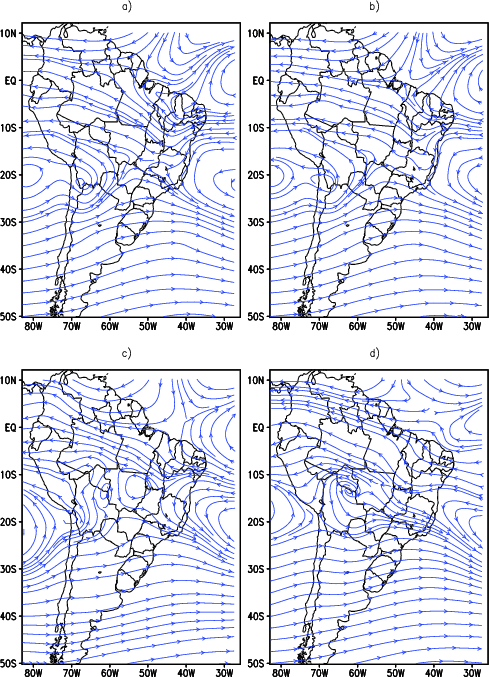
\includegraphics[height=15cm]{./figs/media_corrente_anl_500hPa.png}
\caption{Idem \autoref{fig10}, para o nível de 500 hPa. As unidades estão em ms-1.}
\label{fig14}
\end{figure}

Nos campos de magnitude e direção do vento meridional em 850 hPa e do vento zonal em 250 hPa pode-se observer a presença dos jatos de baixos e altos níveis respectivamente.

A partir da descrição da média da componente meridional em 850 hPa (\autoref{fig15}), é possível identificar o JBN que é caracterizado por ventos de norte/nordeste intensos em baixos níveis canalizados pela topografia dos Andes (bloqueio topográfico). Este tipo de jato fica bem caracterizado na média da reanálise do NCEP, havendo um pequeno sinal de sua atuação na reanálise do CPTEC. No entanto, não há sinal aparente de sua presença nas médias das simulações SAP e CAP. Este fato pode estar associado às caracaterísticas de circulação que foram encontradas nos campos de linha de corrente em 850 hPa (\autoref{fig10}) em que pode-se perceber o contraste existente entre os experimentos e as reanálises. \citeonline{soaresmarengo04} apresentam um estudo de caso JBN à leste dos Andes sobre a AS, em Janeiro de 2003. Neste estudo, os autores identificaram um caso de JBN utilizando a reanálise 2 do NCEP/DOE. Os critérios de Bonner utilizados para a identificação do JBN são aqueles adaptados para AS. A partir destes critério, fica claro que os experimentos SAP e CAP não mostram evidências da atuação do JBN, principalmente porque a componente medional do vento em 850 hPa é de sul com valores menores do 12 ms-1. Soares e Marengo também comparam simulações do modelo Eta de 40 km (com condições de contorno do modelo global do CPTEC e com condições iniciais a análises do NCEP) e mostram que as previsões desse modelo tendem a subestimar os valores da magnitude da componente meridional do vento. Além disto, como trata-se das médias dos campos espaciais, possivelmente este fenômeno observado nas reanálises pode ter sido mascarada nos experimentos. Também, o fato de os experimentos SAP e CAP terem sido interpolados para a grade da reanálise do NCEP, pode penalizar o detalhamento associado à melhor resolução espacial dos experimentos realizados.

Entre outros aspectos que podem ser notados, pode-se citar que os experimentos e a reanálise do NCEP concordam sobre a intensidade do vento sobre a região norte do continente. Neste caso, a reanálise do CPTEC tende a superestimar a intensidade do vento em superfície em relação aos experimentos e reanálise do NCEP. 

\begin{figure}[!hbp]
\centering
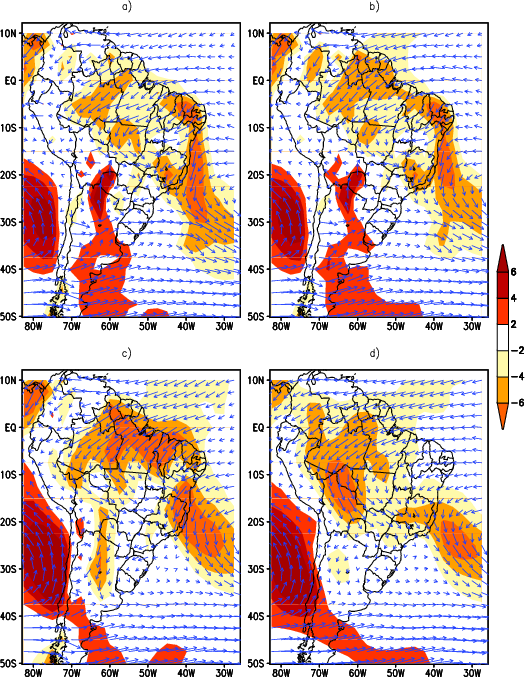
\includegraphics[height=15cm]{./figs/media_vento-meridional_anl_850hPa.png}
\caption{Componente Meridional do vento para o nível de 850 hPa. a) experimento SAP, b) experimento CAP, c) Reanálise CPTEC, d) Reanálise 2 NCEP/DOE. As unidades estão em ms-1.}
\label{fig15}
\end{figure}

Em 250 hPa, os campos da componente zonal do vento são mostrados na \autoref{fig16}. Neste nível, a presença dos Jatos de Altos Nível ao sul do continente é marcante e sua atuação é importante devido à influência que exercem na propagação de frentes atmosféricas e na formação de alguns sistemas convectivos. Os experimentos SAP e CAP, neste nível, apresentam características semelhantes de escoamento, tando em relação à circulação quanto em relação à intensidade. O mesmo ocorre em relação às duas reanálises, sendo que a do NCEP fecha um vórtice (que pode ser visto no campo de linha de corrente da \autoref{fig12}). Este vórtice não é bem caracterizado pelos dois experimentos. 

Observa-se também que a magnitude desta componente do vento simulada pelos experimentos SAP e CAP é mais intensa neste nível, o que também pode ser notado no campo de linha de corrente em 250 hPa (\autoref{fig12}) com gradientes zonais intensos, entre as latitudes de 30ºS e 20ºS. No entanto, a posição e a intensidade dos Jatos é bem definida e coerente entre os quatros campos apresentados na \autoref{fig16}, com a componente zonal do vento apresentando valores máximos (acima de 24 ms-1) em relação às posições climatológicas de 35ºS a 70ºS para o Jato Polar (JP) – embora não mostrado e de 20ºS a 30ºS para o Jato Subtropical (JST). Estes valores podem ser encontrado em \citeonline{reiter69} e \citeonline{riehl69}. 

\begin{figure}[!hbp]
\centering
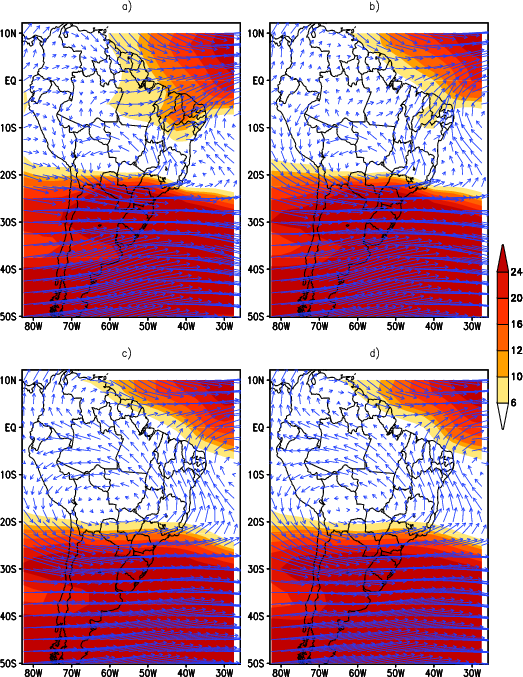
\includegraphics[height=15cm]{./figs/media_vento-zonal_anl_250hPa.png}
\caption{Componente Zonal do vento para o nível de 250 hPa. a) experimento SAP, b) experimento CAP, c) Reanálise CPTEC, d) Reanálise 2 NCEP/DOE. As unidades estão em ms-1.}
\label{fig16}
\end{figure}

\begin{figure}[!hbp]
\centering
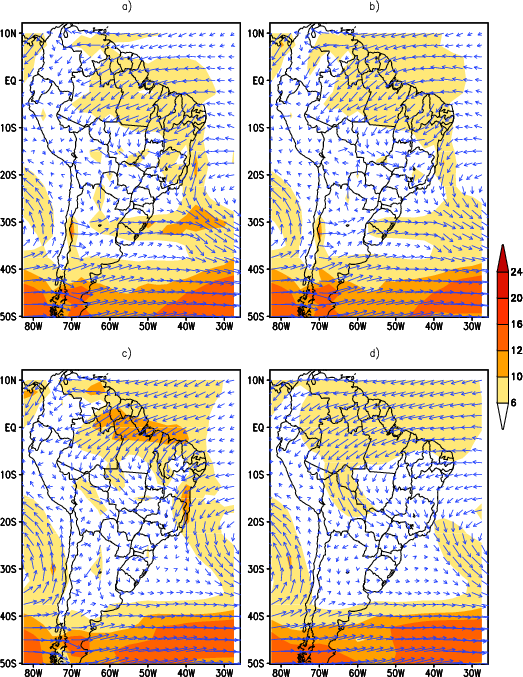
\includegraphics[height=15cm]{./figs/media_ventos_anl_850hPa.png}
\caption{Magnitude e direção do vento ($u+v$) para o nível de 850 hPa. a) experimento SAP, b) experimento CAP, c) Reanálise CPTEC, d) Reanálise 2 NCEP/DOE. As unidades estão em ms-1.}
\label{fig17}
\end{figure}

\begin{figure}[!hbp]
\centering
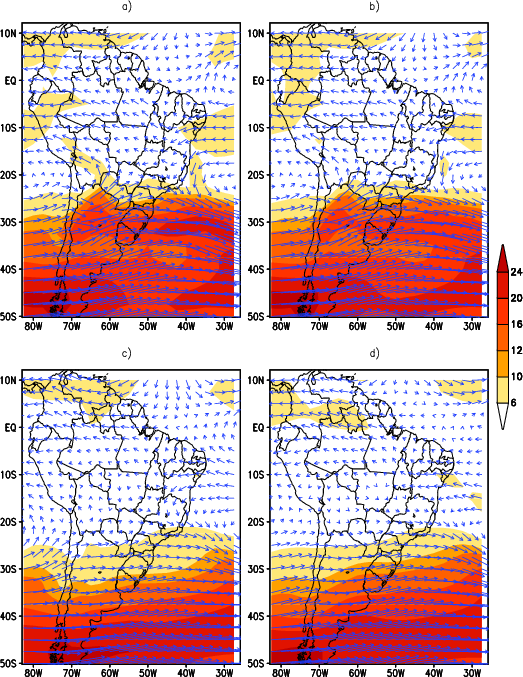
\includegraphics[height=15cm]{./figs/media_ventos_anl_500hPa.png}
\caption{Idem \autoref{fig17}, para o nível de 500 hPa.}
\label{fig18}
\end{figure}

\begin{figure}[!hbp]
\centering
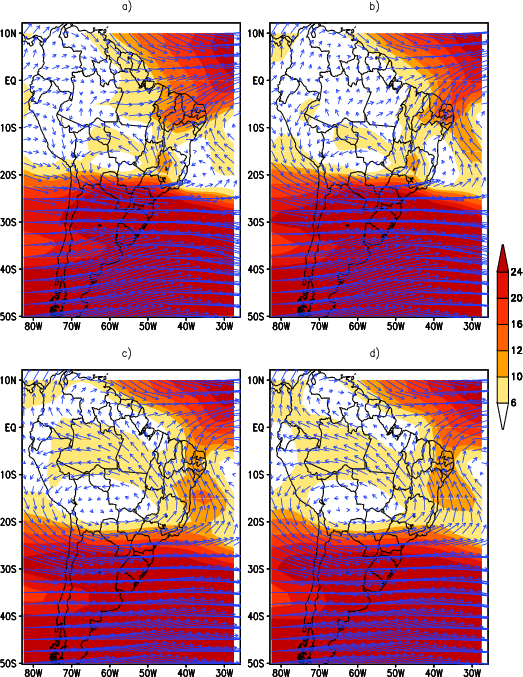
\includegraphics[height=15cm]{./figs/media_ventos_anl_250hPa.png}
\caption{Idem \autoref{fig17}, para o nível de 250 hPa.}
\label{fig19}
\end{figure}

A comparação entre os experimentos e as reanálises do NCEP e do CPTEC para a temperatura do ar, mostra que para os três níveis avaliados (850, 500 e 250 hPa – \autoref{fig20}, \autoref{fig21} e \autoref{fig13}, respectivamente) as temperaturas, em boa parte do continente (aproximadamente entre a faixa de latitudes de -20ºS e 10ºN), tenderam a ser mais quentes (~2ºC a mais do que as reanálises). Estas diferenças também podem ser notadas nas médias dos campos de Altura Geopotencial devido à relação existente (hipsométrica) entre temperatura e a espessura da camada acima.

\begin{figure}[!hbp]
\centering
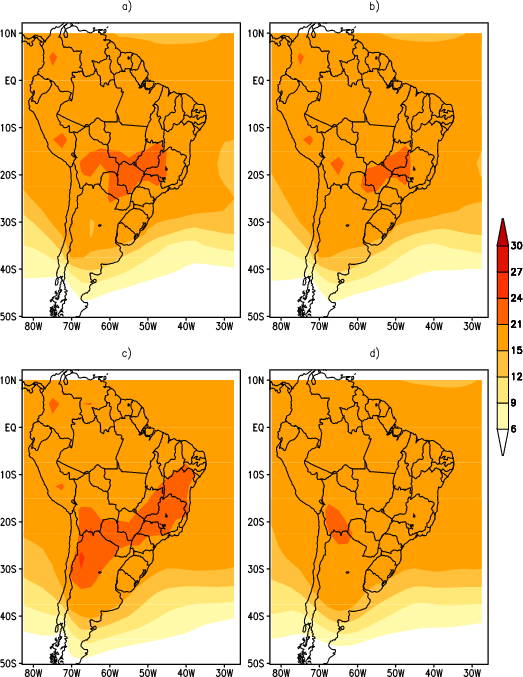
\includegraphics[height=15cm]{./figs/media_temp_anl_850hPa.png}
\caption{Idem \autoref{fig13}, para o nível de 850 hPa.}
\label{fig20}
\end{figure}

\begin{figure}[!hbp]
\centering
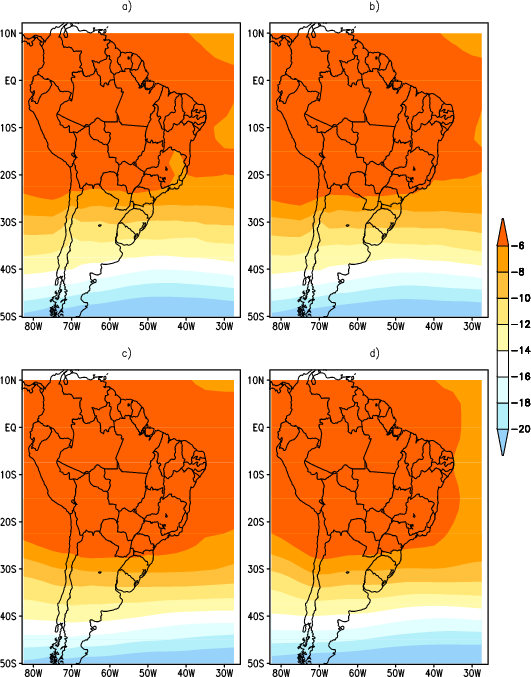
\includegraphics[height=15cm]{./figs/media_temp_anl_500hPa.png}
\caption{Idem \autoref{fig13}, para o nível de 500 hPa.}
\label{fig21}
\end{figure}

Outros campos foram também calculados, como os campos médios de Altura Geopotencial, mas foram omitidos por não apresentarem resultados muito significativos entre os experimentos e em relação às reanálises.

\subsection{Avaliação Espacial e das Séries das Análises (Análises RPSAS X Reanálise NCEP)}
\label{ss:avalesanl}

As figuras a seguir mostram as séries do Viés e do Erro Quadrático Médio das análises em relação à reanálise do NCEP, para os níveis de 850, 500 e 250 hPa para as seguintes variáveis: Altura Geopotencial [mgp], Temperatura do Ar [ºC], Ventos Zonal e Meridional [ms-1] e Umidade Relativa [$\%$], durante 02 e 30 de Janeiro de 2003.

A avaliação das séries temporais das análises do RPSAS em relação às análises do NCEP, mostram que, em geral, os maiores valores de erro (Viés) encontram-se no nível de 250 hPa, para o experimento SAP. O experimento CAP apresenta valores de Viés menores (se comparado com o experimento SAP), sugerindo que a assimilação de precipitação tende a retirar mais o Viés em superfície (850 hPa) e em médios níveis (500 hPa) do que em altos níveis. Esta avaliação é válida para as variáveis dinâmicas do modelo, tais como ventos (zonal e meridional), temperatura e umidade. A altura geopotencial, ao contrário do que se segue para as variáveis dinâmicas, apresenta maiores diferenças de Viés e EQM para o nível de 250 hPa. Isto pode ser explicado pelo fato de que os valores de Viés e EQM da variável Temperatura do Ar apresentarem maiores diferenças entre os experimentos em baixos e médios níveis, 850 e 250 hPa. A avaliação da distribuição espacial do Viés e do EQM reforçam este ponto de vista. 

Para a Altura Geopotencial (\autoref{fig30a} e \autoref{fig30b}), observa-se que os maiores valores de Viés e EQM estão no nível de 250 hPa e sobre a região Sul do Brasil e Argentina. Comparativamente, os experimentos SAP e CAP tenderam a subestimar a altura geométrica do Geopotencial ($~$30 mgp), sendo que o experimento CAP apresentou um distribuição menor do erro do que o experimento SAP. Além disso, neste mesmo nível, o experimento CAP em algumas partes da região de avaliação, removeu o Viés negativo e em outras acabou por superestimar o valor do Viés. Consequentemente, a distribuição espacial do EQM para esta variável também é maior em altos níveis. Em 850 e 500 hPa, o valor do EQM para altura Geopotencial foi menor do que em 250 hPa, nível em que a distribuição espacial do EQM foi maior e acima de 20 mgp.

\begin{figure}[!hbp]
\centering
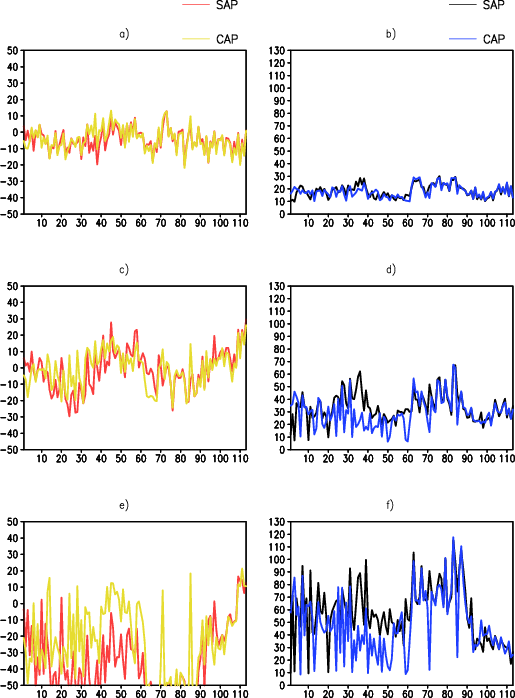
\includegraphics[height=15cm]{./figs/vies_eqm-zgeo.png}
\caption{Viés (coluna da esquerda) e Erro Quadrático Médio (coluna da direita) da Altura Geopotencial [mgp] para os níveis de 850 (primeira linha), 500 (segunda linha) e 250 hPa (terceira linha). As linhas vermelha e preta representam o experimento SAP e as linhas amarela e azul, o experimento CAP. As unidades estão em mgp.}
\label{fig30a}
\end{figure}

\begin{figure}[!hbp]
\centering
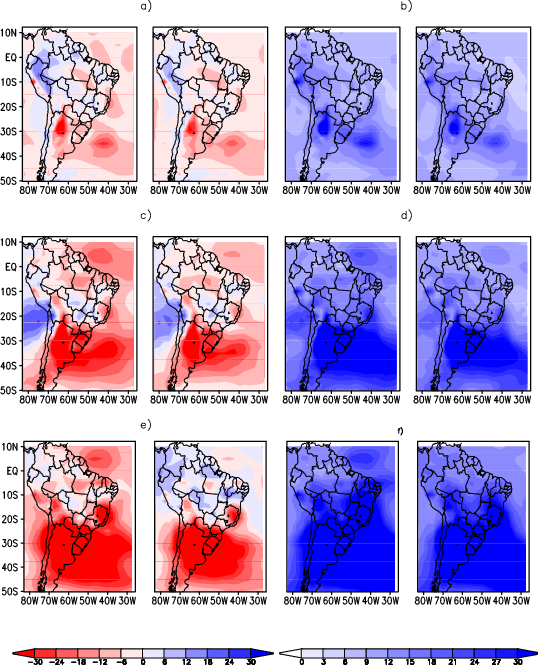
\includegraphics[height=15cm]{./figs/campo_vies_eqm-zgeo.png}
\caption{Viés e EQM espacial da Altura Geopotencial [mgp] para os níveis de a,b) 850 hPa; c,d) 500 hPa e e,f) 250 hPa. As colunas 1 e 3 representam o Viés e o EQM para o experimento SAP, respectivamente. As colunas 2 e 4, representam o Viés e o EQM para o experimento CAP, respectivamente. As unidades estão em mgp.}
\label{fig30b}
\end{figure}

A temperatura, ao contrário do que foi encontrado para a Altura Geopotencial, apresentou maiores valores de Viés e EQM em superfície do que em médios e altos níveis (\autoref{fig31a} e \autoref{fig31b}). Em 850 hPa, a maior parte do Viés concentrou-se na região centro-oeste do Brasil apresentando valores positivos de Viés e em poucos pontos isolados valores negativos, como sobre o a região central da Argentina. Em 500 hPa, os valores de Viés foram menores havendo um deslocamento do Viés positivo da temperatura para a região oeste do continente, porém com valores menores. Sobre a região centro-oeste do continente, os valores negativos de Viés também foram minimizados. Já em 250 hPa, os erros foram bem menore se comparados aos valores de erro em superfície (850 hPa). Neste nível, porém, observa-se que uma pequena tendência de Viés positivo sobre o oceano Atlântico Subtropical. Sobre o Norte da Argentina, e comparativamente ao experimento SAP, o experimento CAP apresentou Viés muito próximo de zero. A distribuição espacial do EQM para a Temperatura Absoluta mostra claramente que os erros mais significativos entre os experimentos foram em baixos níveis.

\begin{figure}[!hbp]
\centering
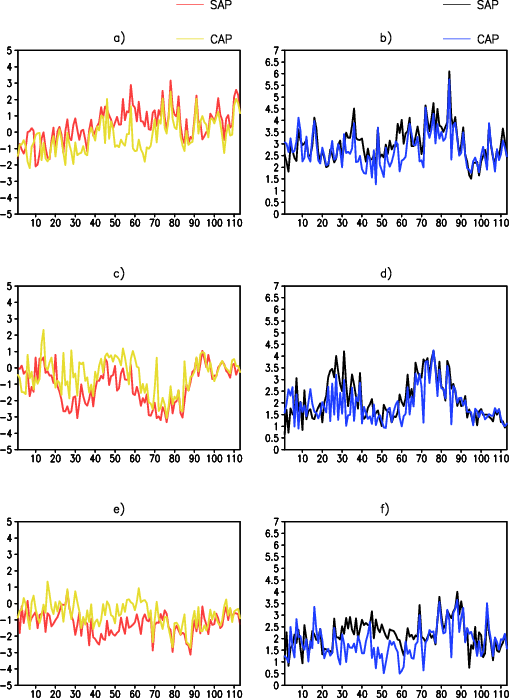
\includegraphics[height=15cm]{./figs/vies_eqm-temp.png}
\caption{Idem \autoref{fig30a}, para a Temperatura do Ar. As unidades estão em ºC.}
\label{fig31a}
\end{figure}

\begin{figure}[!hbp]
\centering
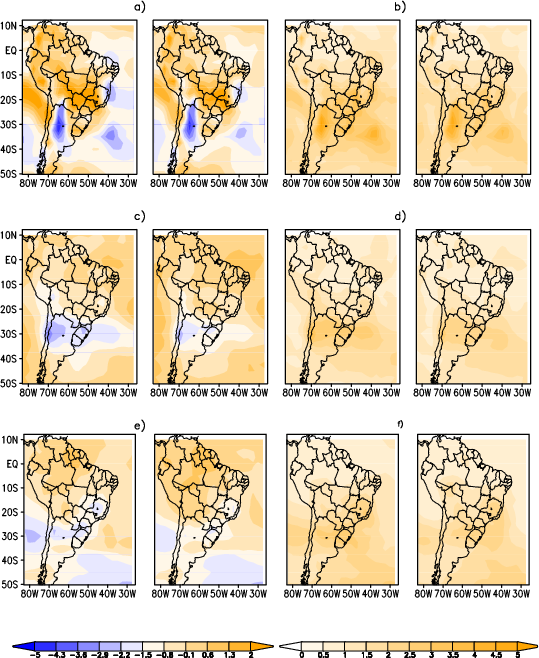
\includegraphics[height=15cm]{./figs/campo_vies_eqm-temp.png}
\caption{Idem \autoref{fig30b}, para a Temperatura do Ar. As unidades estão em ºC.}
\label{fig31b}
\end{figure}

As componentes Zonal e Meridional do vento (\autoref{fig32a} e \autoref{fig32b}, \autoref{fig33a} e \autoref{fig33a} respectivamente) avaliadas, mostram que maiores valores de Viés foram encontradas em 850 hPa e 500 hPa, respectivamente. A distribuição espacial do Viés do vento meridional nestes dois níveis é semelhante entre ambos os experimentos, sendo que o experimento CAP tende a atenuar os valores máximos e mínimos do Viés. Em boa parte do continente, ambos os experimentos tendem a subestimar o valor da componente meridional do vento. Em regiões isoladas (regiões central do continente e norte da Argentina), os experimentos apresentaram valores altos de Viés. Em 250 hPa, os valores de Viés apresentados pelos experimentos tendem a ser atenuados, embora o EQM apresentado por eles seja um pouco maior do que aqueles observados em 500 e 850 hPa. Já os valores de Viés e EQM calculados para os experimentos CAP e SAP para a componente zonal do vento, mostram que há uma tendência maior dos experimentos em superestimar os valores desta componente em altos níveis. Em 500 e 850 hPa, os valores de Viés tendem a ser menores ($\sim$5 ms-1), sendo que sobre o norte da Argentina e sul do Brasil, estes valores são levemente superestimados.

\begin{figure}[!hbp]
\centering
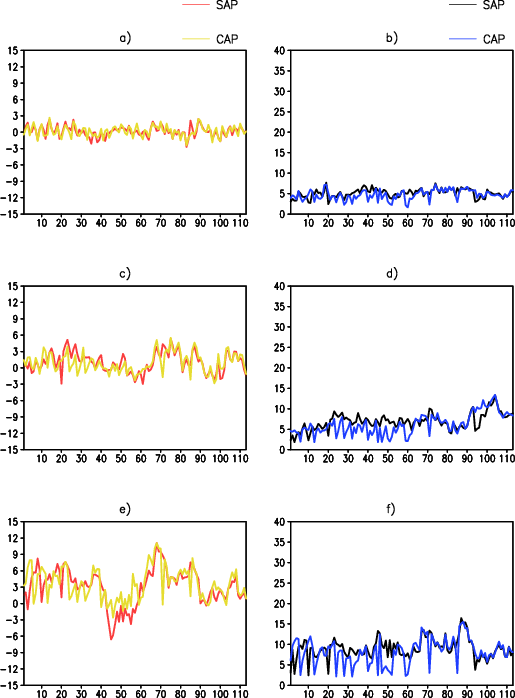
\includegraphics[height=15cm]{./figs/vies_eqm-uvel.png}
\caption{Idem \autoref{fig30a}, para o Vento Zonal. As unidades estão em ms-1.}
\label{fig32a}
\end{figure}

\begin{figure}[!hbp]
\centering
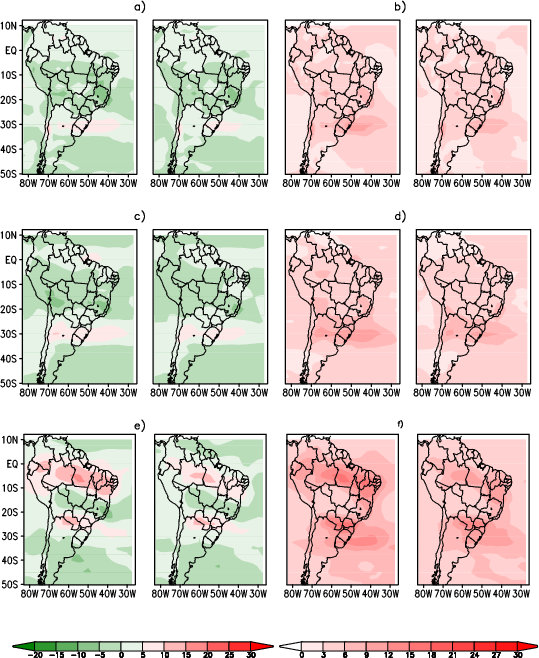
\includegraphics[height=15cm]{./figs/campo_vies_eqm-uvel.png}
\caption{Idem \autoref{fig30b}, para o Vento Zonal. As unidades estão em ms-1.}
\label{fig32b}
\end{figure}

\begin{figure}[!hbp]
\centering
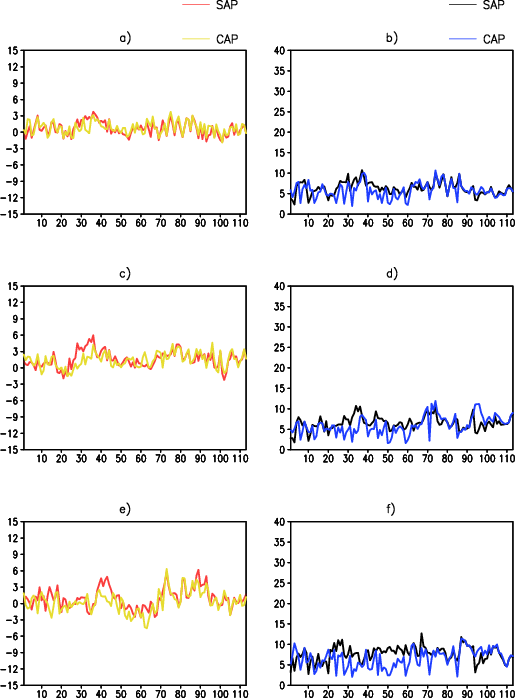
\includegraphics[height=15cm]{./figs/vies_eqm-vvel.png}
\caption{Idem \autoref{fig30a}, para Vento Meridional. As unidades estão em ms-1.}
\label{fig33a}
\end{figure}

\begin{figure}[!hbp]
\centering
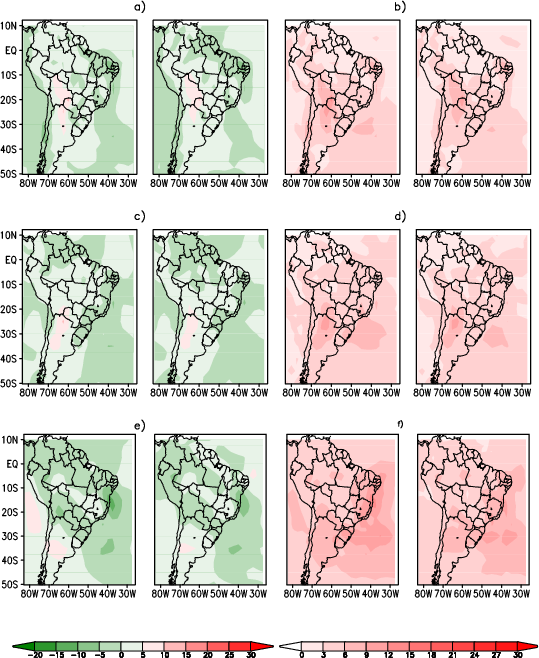
\includegraphics[height=15cm]{./figs/campo_vies_eqm-vvel.png}
\caption{Idem \autoref{fig30b}, para Vento Meridional. As unidades estão em ms-1.}
\label{fig33b}
\end{figure}

A avaliação do Viés e EQM da umidade relativa para os níveis de 850, 500 e 250 hPa - \autoref{fig34a} e \autoref{fig34b}, mostra que em níveis médios (500 hPa)), os experimentos SAP e CAP foram menos tendenciosos em superestimar ou subestimar os valores relativos de umidade. Neste nível, foram encontrados menores valores de EQM. Em relação os níveis de 850 hPa e 500 hPa, houve maior tendencia dos experimentos em subestimar a umidade do ar, sendo que novamente o experimento CAP atenuou os valores do Viés e do EQM.

\begin{figure}[!hbp]
\centering
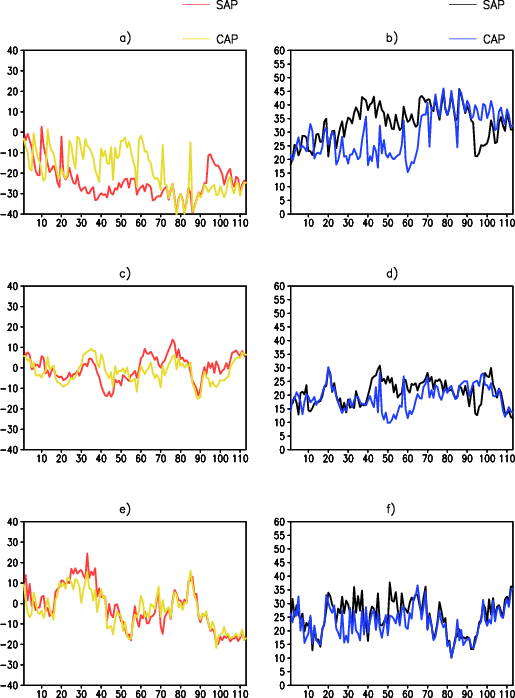
\includegraphics[height=15cm]{./figs/vies_eqm-umrl.png}
\caption{Idem \autoref{fig30a}, para a Umidade Relativa [\%].}
\label{fig34a}
\end{figure}

\begin{figure}[!hbp]
\centering
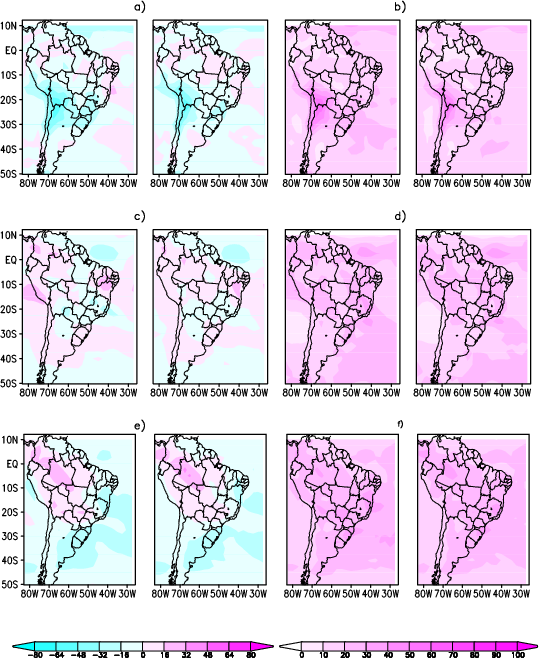
\includegraphics[height=15cm]{./figs/campo_vies_eqm-umrl.png}
\caption{Idem \autoref{fig30b}, para a Umidade Relativa [\%].}
\label{fig34b}
\end{figure}

\subsection{Avaliação da Temperatura e Umidade do Solo (SAP X CAP)}
\label{ss:avaltempumi}

Em relação à temperatura e umidade do solo, a versão do modelo Eta utilizada nos experimentos desta dissertação utiliza o modelo de superfície NOAH para o cálculo destas variáveis. Neste caso as condições iniciais de temperatura e umidade do solo são provenientes do modelo Global do CPTEC T126L28 e são atualizadas pelo modelo NOAH. A \autoref{fig50} mostra a série temporal da umidade do solo durante o período de assimilação (de 02 a 30 de Janeiro) do modelo Eta bem como os campos médios.

\begin{figure}[!hbp]
\centering
\includegraphics[height=15cm]{./figs/serie_umidade_solo-ANL.png}
\caption{a) e b) Série temporal da umidade do solo para a área de estudo (BP) e América do Sul (AS), respectivamente. c) e d) Campos médios da umidade do solo para os experimentos SAP e CAP, respectivamente. Linhas vermelha e preta representam o experimento SAP. Linhas amarela e azul, representam o experimento CAP. As unidades estão em kg/s-1.}
\label{fig50}
\end{figure}

Nesta figura são mostradas as séries temporais da umidade do solo (entre 0 e 10 cm - primeira camada) (a) para os experimentos SAP e CAP, tanto para o domínio de integração do modelo (AS) quanto para a região de estudo (BP). Comparando-se os experimentos SAP e CAP, nota-se que o experimento CAP apresenta valores de umidade mais elevados do que o experimento SAP. Numericamente, a maior diferença entre as séries temporais é de ~0,08 kg/m-2.

Em relação à temperatura do solo (\autoref{fig51}), também observou-se que o experimento CAP apresentou valores diferentes em relação ao experimento SAP. Em média, estes valores não diferem muito (imagens ``c'' e ``d'' da \autoref{fig51}), sendo que menores valores podem ser encontrados na série do experimento CAP (linhas amarela e azul das imagens ``a'' e ``b''), tanto para a área de estudo (BP) quanto para o domínio de integração (AS).

\begin{figure}[!hbp]
\centering
\includegraphics[height=15cm]{./figs/serie_temperatura_solo-ANL.png}
\caption{Idem \autoref{fig50}, para a Temperatura do Solo. As unidades estão em ºC.}
\label{fig51}
\end{figure}

\subsection{Avaliação das Previsões (Previsões Eta X Observações)}
\label{ss:avalprev}

Neste tópico é feito uma avaliação das prevsiões de 6 horas do modelo Eta (geradas a partir das análises avaliadas na seção anterior) em comparação com os dados observacionais e estimados do SALLJEX, GPCP e TRMM.

Na \autoref{fig52} são mostradas as séries das previsões de 6 horas de precipitação dos experimentos SAP (linhas com sinal de cruz), CAP (linhas com bolas abertas),  e as séries de precipitação do GPCP (linhas com bolas fechadas),  SALLJEX (linhas com quadrados abertos) e TRMM (linhas com quadrados fechados). São mostrados também os campos médios destas séries de precipitação.

Comparando-se os campos de previsão de 6 horas de precipitação produzidos pelo modelo Eta a partir dos campos dos experimentos SAP e CAP em relação ao GPCP, SALLJEX e TRMM, observa-se que os campos de precipitação do produzidos pelo experimento CAP apresenta um nível de detalhamento e distribuição da precipitação um pouco maior do que aquele apresentado pelo experimento SAP. Em comparação com o GPCP e SALLJEX (que apresentam campos similares, porém com níveis de detalhamento sensivelmente diferentes), os experimentos CAP e SAP subestimaram a quantidade de precipitação em boa parte do domínio, embora os padrões de precipitação apresentados não sejam muito divergentes. A precipitação do TRMM é a que mais se apresentou deficiente na representação do campo e nos valores acumulados. Isto se deve ao fato de que em alguns horários não havia informação disponível dos campos de precipitação, o que acabou contrinuindo para que a média apresentada pelo TRMM fosse penalisada. Os projetos SALLJEX e GPCP, incluem informações de alta resolução espacial e temporal, especialmente o GPCP. Este tipo de amostragem espaço-temporal é importante porque auxiliam em estudos diagnósticos e de modelagem, uma vez que a sua inclusão nos modelos pode colaborar para os prognósticos produzidos sejam mais realísticos. 

As séries temporais dos experimentos, sobre a AS (\autoref{fig52} - imagem ``b'') mostram claramente a quantidade de observações de precipitação é muito importante para a composição de uma campo de previsão de precipitação mais realístico. As diferenças entre as alturas pluviométricas entre os experimentos e o GPCP/SALLJEX chegam a ser da ordem de 10 mm em alguns dias. No entorno do dia 23 de Janeiro, por exemplo, nota-se que os experimentos SAP e CAP subestimaram a altura pluviométrica, sendo que o experimento SAP forneceu a pior estimativa.  Em relação ao experimento SAP, o experimento CAP apresentou um valor razoável da altura pluviométrica para este dia porque assimilou as informações de precipitação do TRMM, reduzindo aquela diferença de 10 mm entre as séries para aproximadamente 4 mm. Por outro lado, dentro da região de estudos (denotada por BP, na imagem ``a'' da \autoref{fig52}), nota-se que o experimento CAP apresentou maior quantidade de precipitação para o dia 22. Observa-se que o experimento CAP apresenta uma altura pluviométrica de 10 mm, sendo que para o domínio total (denotado por AS na imagem ``b''), neste mesmo dia o SALLJEX apresenta uma altura de aproximadamente 14 mm. Esta diferença se deve porque o cálculo realiza para a área AS condidera todo o campo de precipitação, em que há algumas regiões onde os experimentos SAP e CAP foram piores. Na área BP, com uma regiãi reduzida, onde inclusive o TRMM apresenta alturas pluviométricas melhores, essa diferença tende a diminuir entre os experimentos e as precipitações observadas. Isto pode estar relacionado ao fato de que a assimilação de precipitação naturalmente tende a suprir maiores informações para o modelo. No entanto, como foram assimiladas somente estimativas do TRMM, a previsão de precipitação fica atrelada à qualidade dos campos de precipitação assimilados. 

\begin{figure}[!hbp]
\centering
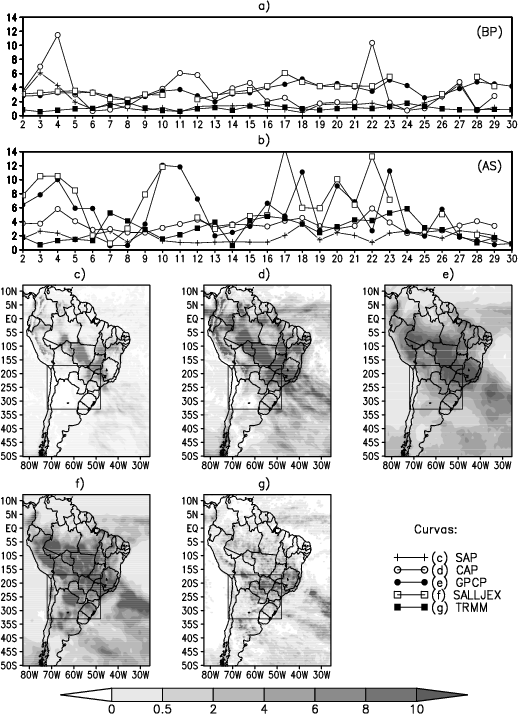
\includegraphics[height=15cm]{./figs/serie_precipitacao-FCT06h.png}
\caption{Seríes das previsões de 6 horas de precipitação. Em a) séries do modelo Eta (linhas vermelha – experimento SAP e amarela – experimento CAP), e GPCP (linha verde) para a região de avaliação destacada nas figuras ``c'', ``d'' e ``e''. Em b) Idem ``a'' para a AS. Em c), d) e e) os campos médios de precipitação para o experimentos SAP, CAP e GPCP. As unidades estão em mm/dia.}
\label{fig52}
\end{figure}

\section{Avaliação do \textit{Skill} do modelo Eta para as previsões de 6 a 24 horas}
\label{ss:avalskill}

Na \autoref{fig53} apresenta-se o Viés, EQM e CA da altura geopotencial para os horários das 00Z (coluna da esquerda) e 12Z (coluna da direita) para as previsões de 0 a 24 horas, no nível de 850 hPa. No geral nota-se que o experimento CAP apresenta resultados um pouco melhores no horário das 00Z durante 0 e 12 horas de previsão (figuras da coluna da esquerda) do que no horário das 12Z. No entanto, às 12Z (figuras da coluna direita) nota-se que entre 12 e 18 horas de previsão o experimento CAP apresenta resultados um pouco melhores. Isso pode ser devido ao fato de que às 12Z a quantidade de observações sinótica é um pouco mais abundante do que às 00Z. Além disso, este resultado indica que o modelo se ajustou aos dados de precipitação assimilados, se comparado com o viés presente em 6 horas de previsão e em comparação com o experimento de controle SAP, que neste mesmo horário apresenta viés quase igual a zero. Em relação ao desempenho, embora os valores de CA se apresentem aquém em relação ao que se conhece do modelo operacional Eta do CPTEC - mas considerando-se a metodologia apresentada, nota-se que o desempenho do experimento CAP, na média, foi melhor no horário das 12Z do que às 00Z. Novamente, isto pode ser devido ao fato de haver uma maior abundância de dados sinóticos assimilados na análise das 12Z, o que levou o modelo a se ajustar mais rapidamente aos dados de precipitação assimilados pelo Eta.

\begin{figure}[!hbp]
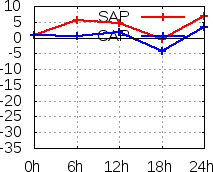
\includegraphics[height=5.5cm]{./figs/VIES850zgeo0Z.png}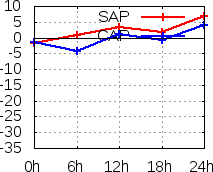
\includegraphics[height=5.5cm]{./figs/VIES850zgeo12Z.png}
\includegraphics[height=5.5cm]{./figs/EQMzgeo0Z.png}\includegraphics[height=5.5cm]{./figs/EQMzgeo12Z.png}
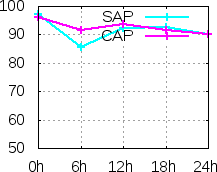
\includegraphics[height=5.5cm]{./figs/CA850zgeo0Z.png}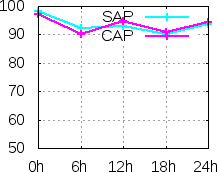
\includegraphics[height=5.5cm]{./figs/CA850zgeo12Z.png}
\caption{Viés, EQM e CA para a variável altura geopotencial em 850 hPa. A coluna da esquerda mostra os valores das medidas para o horário das 00Z. A coluna da esquerda mostra os valores das medidas para o horário das 12Z.}
\label{fig53}
\end{figure}

A próxima figura (\autoref{fig54}) mostra os valores dos índices estatísticos para a altura geopotencial no nível de 500 hPa.

\begin{figure}[!hbp]
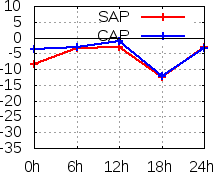
\includegraphics[height=5.5cm]{./figs/VIES500zgeo0Z.png}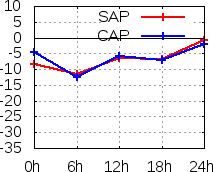
\includegraphics[height=5.5cm]{./figs/VIES500zgeo12Z.png}
\includegraphics[height=5.5cm]{./figs/EQMzgeo0Z.png}\includegraphics[height=5.5cm]{./figs/EQMzgeo0Z.png}
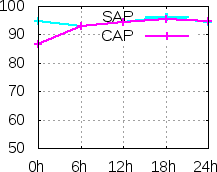
\includegraphics[height=5.5cm]{./figs/CA500zgeo0Z.png}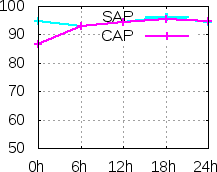
\includegraphics[height=5.5cm]{./figs/CA500zgeo0Z.png}
\caption{Viés, EQM e CA para a variável altura geopotencial em 500 hPa. A coluna da esquerda mostra os valores das medidas para o horário das 00Z. A coluna da esquerda mostra os valores das medidas para o horário das 12Z.}
\label{fig54}
\end{figure}

Analisando-se o a altura geopotencial no nível de 500 hPa, observa-se que os valores de viés para ambos os experimentos tendem a ser negativos durante todo o período de previsão (de 0 a 24 horas). Isto significa os experimentos SAP e CAP subestimaram o valor do geopotencial em níveis médios fazendo com que os valores do EQM aumentassem de 10 mgp para valores entre 20 e 30 mgp. Observa-se um distanciamento sensível dos valores apresentados pelos experi-mentos em relação à Reanálise em 18 horas de previsão, no horário das 00Z. Este diferença é refletida nos valores do EQM, mas não afeta o desempenho geral do experimento CAP que, durante as 24 horas de previsão, apresentou pequena diferença em relação ao experimento de controle SAP. No horário das 12Z, o experimento CAP mostra-se melhor durante as 24 horas de previsão. Aparentemente, a quantidade de dados sinóticos assimilados, influencia a composição do campo de geopotencial pelo modelo, sendo (a \textit{priori}) um indicativo da necessidade de mais dados de observação para a melhoria da condição inicial do modelo, tal como foi verificado por \citeonline{andreolietal08}. Tanto em 850 hPa (não mostrado) quanto em 500 hPa (\autoref{fig54}), para o horário das 12Z, nota-se uma convergência dos valores de CA em 12 horas de previsão, o que pode ser atribuído a uma falha no campo de precipitação associado (um dado ausente no horário da previsão).

Em todos os dois experimentos analisados (SAP e CAP), utilizou-se como condição inicial a análise do NCEP. Posteriormente, após o primeiro ciclo de previsões, o próprio sistema Eta+RPSAS gerou a análise utilizada nos ciclos subsequentes. Na avaliação destes resultados utiliza-se também um produto puramente de modelagem que é a Reanálise. Comparar dados de previsão, que embora sejam corrigidos por observações sinóticas, mas que tendem a se distanciar da verdade com o passar do tempo, pode ser tendencioso no sentido de se onerar a qualidade das previsões dos experimentos e dar mais peso à modelagem. Isso pode acontecer porque a Reanálise se utiliza de dados modelados para reproduzir o estado passado da atmosfera, quase que de forma inversa ao que é feito com a previsão de tempo, onde se utiliza dados observados para se representar o estado presente ou futuro da atmosfera. Com isso, o produto que se obtém da Reanálise possui uma qualidade muito grande porque nela está contida a maior quantidade possível de dados observados que, em comparação à realidade dos experimentos, pode não ser verdade.

A seguir (\autoref{fig55}) são apresentados os resultados do Viés, do EQM e da CA para a temperatura do ar.

\begin{figure}[!hbp]
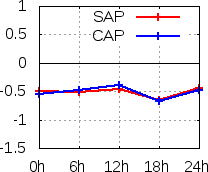
\includegraphics[height=5.5cm]{./figs/VIES850temp0Z.png}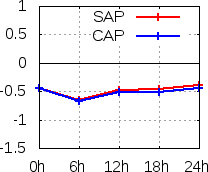
\includegraphics[height=5.5cm]{./figs/VIES850temp12Z.png}
\includegraphics[height=5.5cm]{./figs/EQMtemp0Z.png}\includegraphics[height=5.5cm]{./figs/EQMtemp12Z.png}
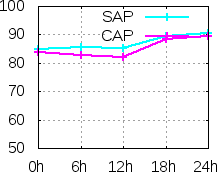
\includegraphics[height=5.5cm]{./figs/CA850temp0Z.png}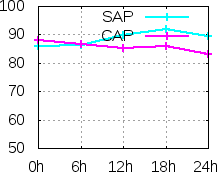
\includegraphics[height=5.5cm]{./figs/CA850temp12Z.png}
\caption{Viés, EQM e CA para a variável temperatura do ar em 850 hPa. A coluna da esquerda mostra os valores das medidas para o horário das 00Z. A coluna da esquerda mostra os valores das medidas para o horário das 12Z.}
\label{fig55}
\end{figure}

A avaliação dos índices estatísticos considerados para a variável temperatura em 850 hPa, sugere que, no geral, o experimento CAP tende a subestimar mais os valores de temperatura ao longo de 24 horas de previsão, tanto às 00Z quanto às 12Z do que o experimento SAP. Este resultado se reflete diretamente nos valores do EQM, principalmente durante as 12 primeiras horas de previsão. Este resultado pode ser associado ao fato de que há menos observações de temperatura no horário das 00Z do que no horário das 12Z. Outro fator que pode ser associado a este resultado é a dependência de que a precipitação tem dos processos de escala de subgrade, seja na liberação de calor latente ou na modulação do perfil vertical de umidade, o qual a temperatura está associada.

A assimilação de precipitação pelo modelo Eta é um processo de inicialização física, onde as variáveis prognósticas do modelo são inicializadas de acordo com as alterações nos perfis verticais de calor e umidade. Estes perfis são alterados quando se compara a precipitação produzida pelo modelo em relação à precipitação observada (conforme explicado na \autoref{tab03}). A temperatura é uma das variáveis que são diretamente influenciadas pelas alterações nos perfis de calor e umidade, devido à sua condição de referência no esquema de convecção. 

A CA da temperatura para o horário das 00Z é menor para o experimento CAP nas 12 primeiras horas de previsão e tendem a ser maior nas últimas 12 horas, em comparação ao experimento SAP. No horário das 12Z observa-se o contrário, sendo o experimento CAP melhor do que o experimento SAP nas 12 primeiras horas de previsão.

Os gráficos da \autoref{fig56} e \autoref{fig57}, mostram os valores dos índices de Viés e EQM para a temperatura do ar nos níveis de 500 e 250 hPa. Em médios e altos níveis, observa-se que o viés da temperatura tende a apresentar um comportamento semelhante ao apresentado em baixos níveis, reforçando a idéia de que a temperatura é sensível às alteração de calor e umidade. No entanto, enquanto que em médios níveis, no horário das 12Z o EQM da temperatura tende a ser pequeno, em altos níveis este erro é muito grande e chega a ser uma ordem de grandeza maior. Em geral, observa-se que o experimento CAP subestima menos os valores de temperatura do que o experimento SAP. A CA da temperatura para esses níveis foi omitida por não apresentar resultados relevantes.
     
\begin{figure}[!hbp]
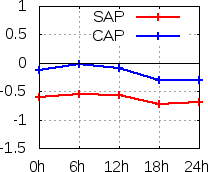
\includegraphics[height=5.5cm]{./figs/VIES500temp0Z.png}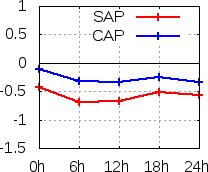
\includegraphics[height=5.5cm]{./figs/VIES500temp12Z.png}
\includegraphics[height=5.5cm]{./figs/EQMtemp0Z.png}\includegraphics[height=5.5cm]{./figs/EQMtemp12Z.png}
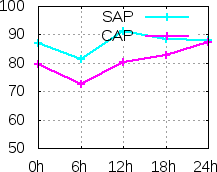
\includegraphics[height=5.5cm]{./figs/CA500temp0Z.png}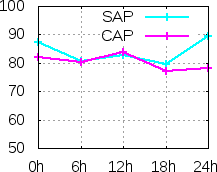
\includegraphics[height=5.5cm]{./figs/CA500temp12Z.png}
\caption{Viés, EQM e CA para a variável temperatura do ar em 500 hPa. A coluna da esquerda mostra os valores das medidas para o horário das 00Z. A coluna da esquerda mostra os valores das medidas para o horário das 12Z.}
\label{fig56}
\end{figure}

\begin{figure}[!hbp]
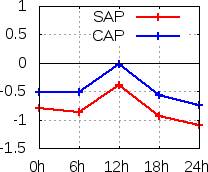
\includegraphics[height=5.5cm]{./figs/VIES250temp0Z.png}\includegraphics[height=5.5cm]{./figs/VIES250temp12Z.png}
\includegraphics[height=5.5cm]{./figs/EQMtemp0Z.png}\includegraphics[height=5.5cm]{./figs/EQMtemp12Z.png}
\includegraphics[height=5.5cm]{./figs/CA250temp0Z.png}\includegraphics[height=5.5cm]{./figs/CA250temp12Z.png}
\caption{Viés, EQM e CA para a variável temperatura do ar em 250 hPa. A coluna da esquerda mostra os valores das medidas para o horário das 00Z. A coluna da esquerda mostra os valores das medidas para o horário das 12Z.}
\label{fig57}
\end{figure}
